\chapter{绪论:交通和数据}

当前人类文明已经进入了所谓的“信息时代”,数据已经渗透进我们社会生产、生活的方方面面,交通领域也不例外。
作为一门工程学科,交通领域的相关专业,如交通工程、交通运输、交通安全等,都遵循“发现问题、分析问题解决问题”的逻辑步骤,在每一个步骤数据都发挥决定性的作用。
本章对交通和数据的关系进行概括的介绍。

\section{什么是数据?}

“\emph{数据}”这个词我们在日常生活中已经广泛使用,但它的来源和确切含义却并不广为人知。
事实上这个词语具有丰富的内涵,了解它不只是满足我们的好奇心,更是让我们能真正意识到它的\emph{重要意义}。中文的“数据”一词翻译自英文单词“data”,按照《牛津字典》的解释,它至少包含两层含义:
\begin{itemize}
    \item 计算机可以操作的数值、字母、符号,能够以磁、光、电、机械的形式存储和传输。
    \item 假设成立或验证成立的\emph{事实},作为进一步推理和计算的基础。\sidenote{things known or assumed as facts, making the basis of reasoning or calculation.}
\end{itemize}
可以看到第一层含义更贴近我们日常用语习惯,但第二层含义才是“data”这个单词的真正来源。

\begin{marginfigure}[-10cm]

\includegraphics[width=\linewidth]{images/spqr.png}
\caption{罗马共和国的标志——SPQR(Senatus PopulusQue Romanus),“罗马的元老院和人民”。}
\end{marginfigure}

英文单词“data”来源于\emph{拉丁语}%
\sidenote{拉丁语是古罗马文明的语言,是意大利语、西班牙语、法语的祖先。罗马帝国灭亡后在很长时间内仍然是欧洲各国进行宗教、文化、科技交流的通用语言。}%
这门古老的语言,原型是拉丁语动词原型“dare”,英文翻译“to give”,意为“给”;按照拉丁语的语法,“dare”的被动语态分词是“datum”,英文翻译“to be given”,意为“被给”;进一步分词名词化,“datum”可以解释为“thing to be given”,意为“被给的东西”。
17世纪中期欧洲哲学家开始在著作中用“datum”一词表达讨论中已经“\emph{给定(given)}”的前提条件,在拉丁语中“datum”作为名词是中性单数,因此对应的复数形式就是“data”。

从来源可以看出,“data”一词实际上是一个哲学概念,是我们探索未知的已知基础。
他的形式并不局限于数字,可以以任何方式存在,例如文字、图片、符号等等;他的重要性和广泛性也远超越交通领域、甚至远远超越了工程技术、自然科学,进入人文、艺术、哲学范畴,
因此一经问世快速被各个领域采纳。
该词汇在书籍中使用比例的变化情况如图\ref{fig:data-trend}所示。
当然,随着计算机技术的发展各种“data”的表示方式逐渐\emph{数字化},因此今天我们可以把“数据”理解为:以数字形式存在的\emph{证据}。

\begin{figure*}
    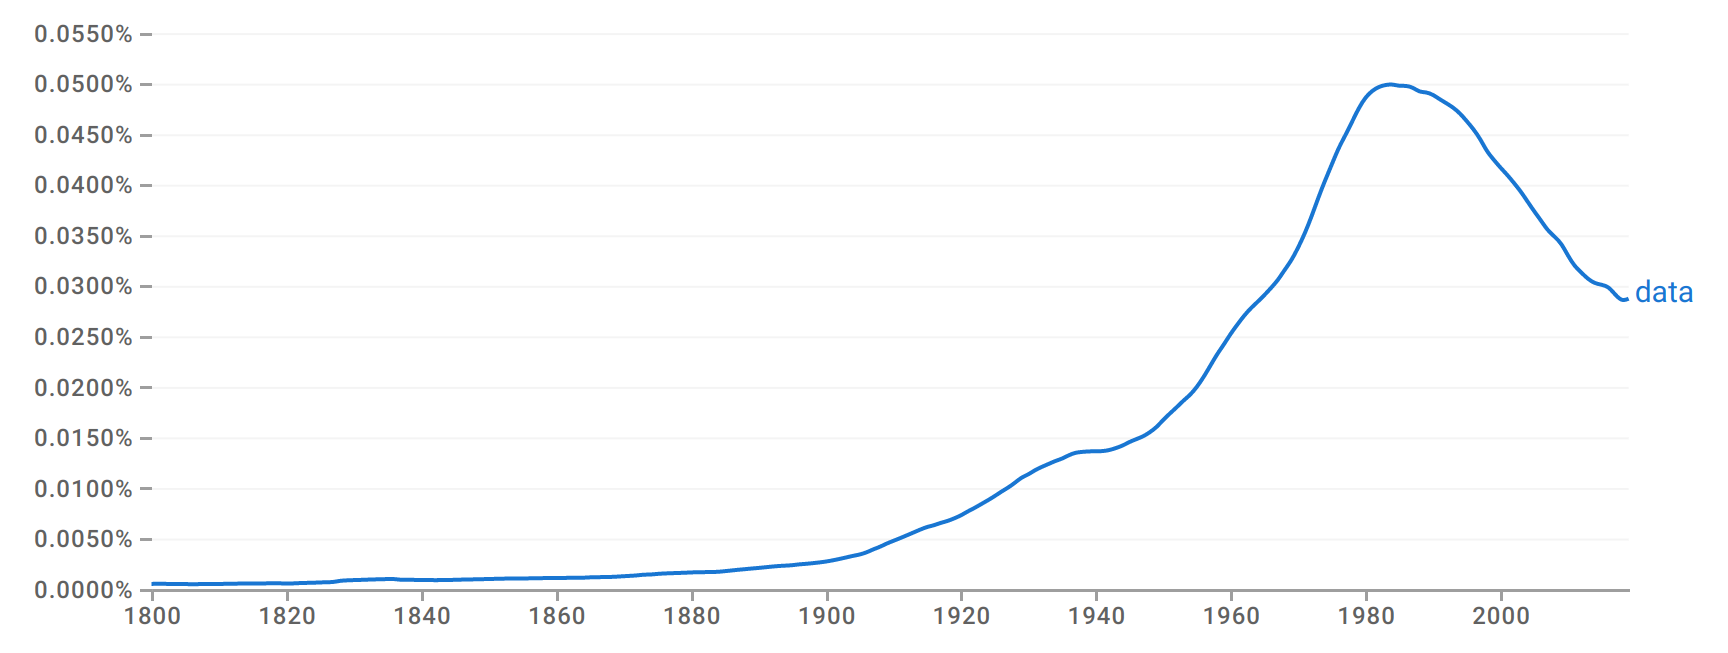
\includegraphics[width=\linewidth]{images/data-vocabulary-trend.png}
    \caption{英文书籍中单词“data”使用频率的变化,数据来自Google Book}
    \label{fig:data-trend}
\end{figure*}
